The groundlaying principles of the Smartsoft Architecture will be pointed out in the following
Sections. A generall overview of how components work together with the sequencer and the instruction planner will be discussed.
Aswell as the placment of the code (which machine runs which part of the software and also how are they connected).

\section{SmartSoft}
Smartsoft is designed as a Development Framwork for Robots to operate in multiple Situations.
Therefor it consists multiple abstraction Layers that base on the principle of
locality. \\
The general Idea is that a Robot should be able to handle as much work as it is locally enabled to do.
Just when an Error occours that the Robot is unable to fix by itself it will escalate the Problem to the next higher instance.
\begin{figure}[h]
\centering
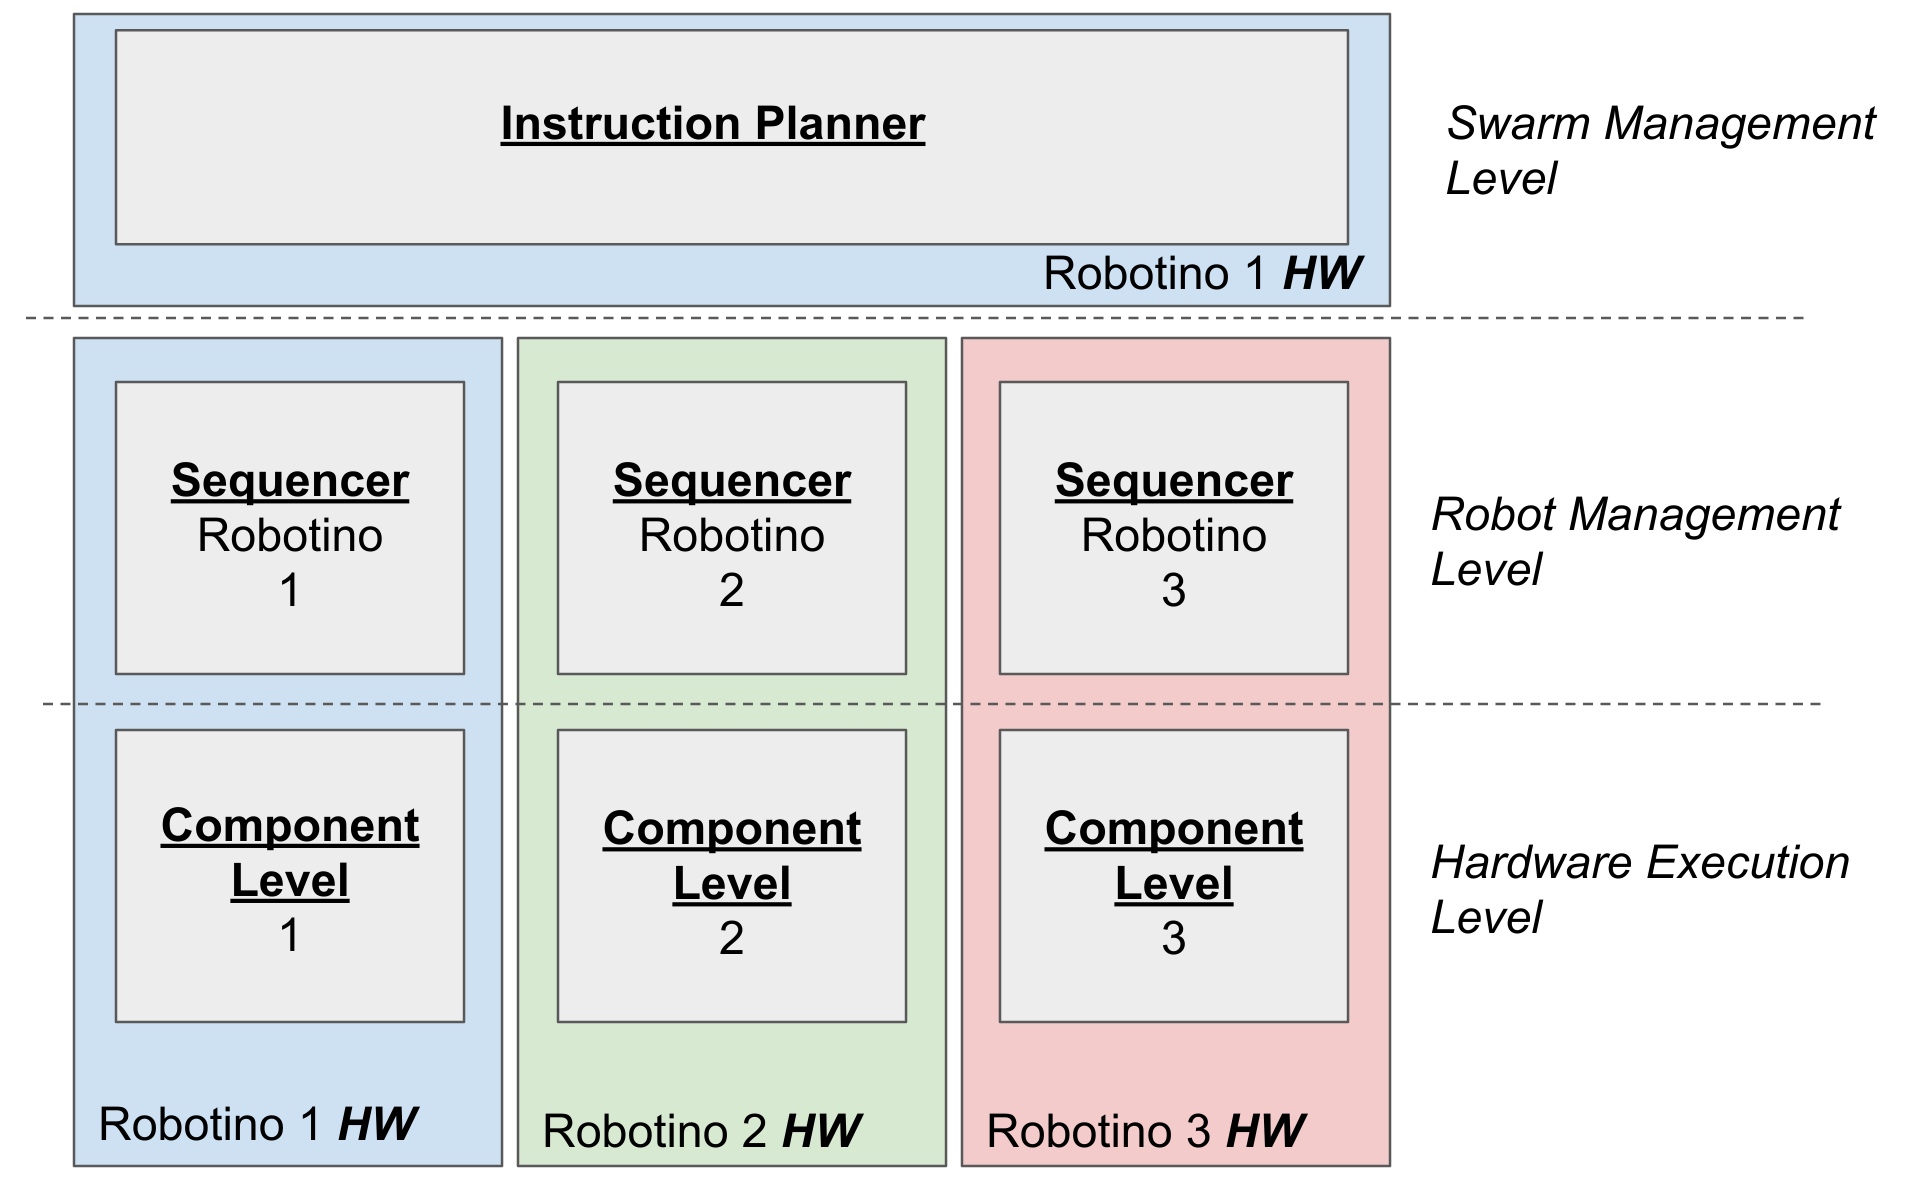
\includegraphics[scale=0.23]{pic/architecture2018.png}
\caption{Arrangement of Components in Architecture}
\label{fig:architecture_overview}
\end{figure}

    \subsection{Instruction Planner}
    \subsection{Sequencer}
    \subsection{Components}
    \subsection{Robots}
    \subsection{Refbox}
